% Created by tikzDevice version 0.7.0 on 2014-06-17 19:18:58
% !TEX encoding = UTF-8 Unicode
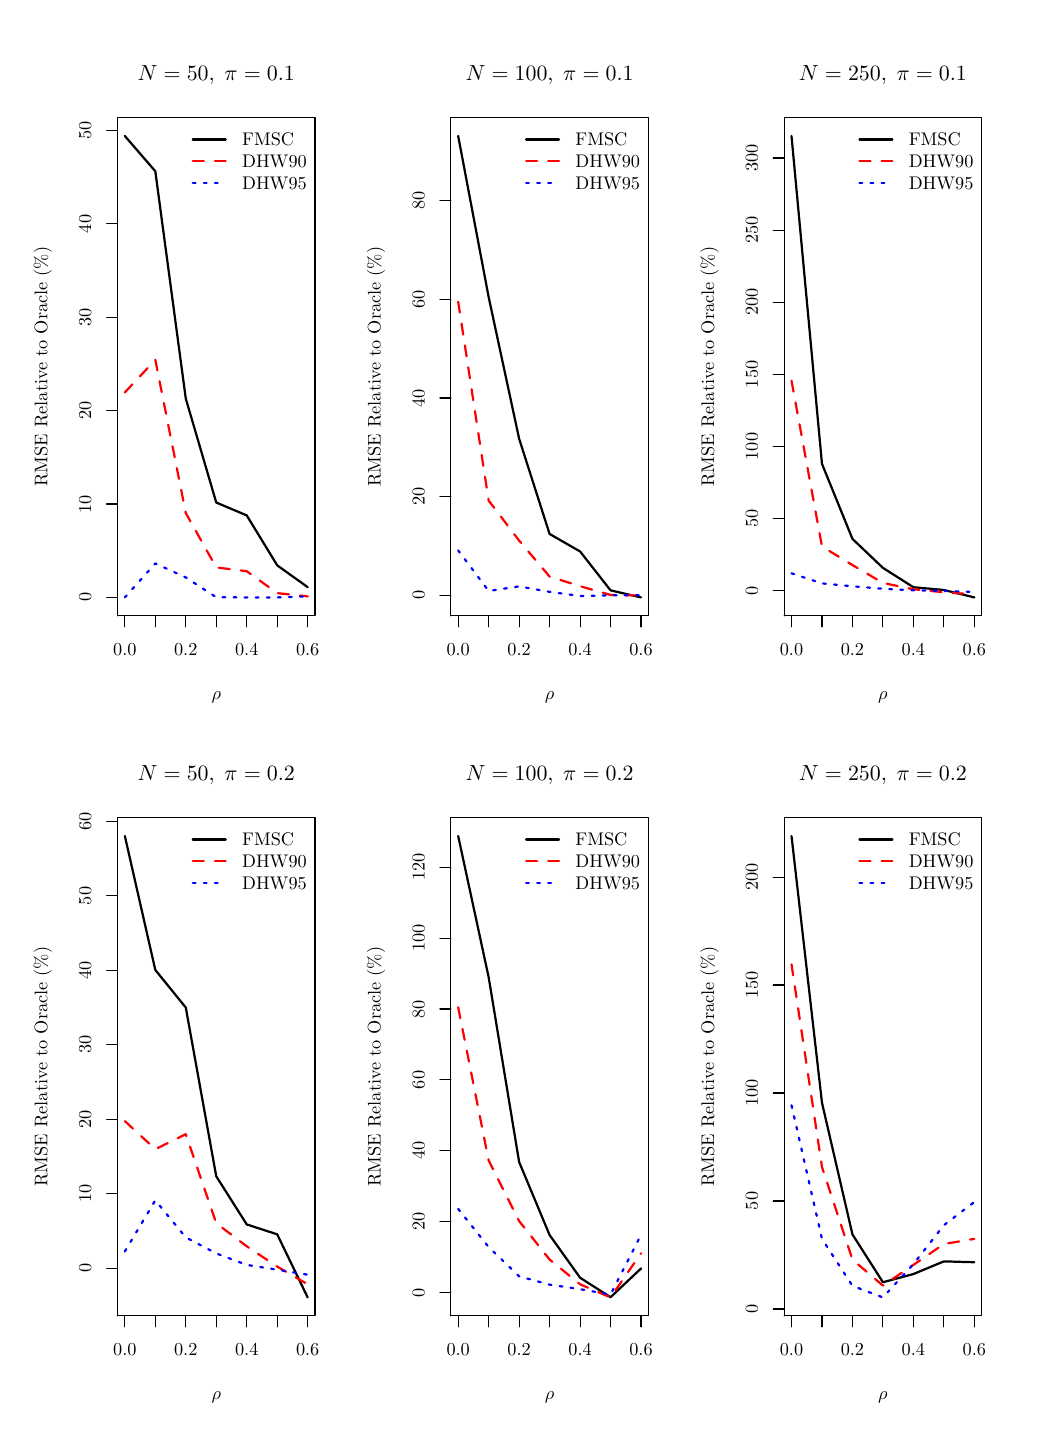
\begin{tikzpicture}[x=1pt,y=1pt]
\definecolor[named]{fillColor}{rgb}{1.00,1.00,1.00}
\path[use as bounding box,fill=fillColor,fill opacity=0.00] (0,0) rectangle (361.35,505.89);
\begin{scope}
\path[clip] ( 32.47,293.34) rectangle (103.82,473.42);
\definecolor[named]{drawColor}{rgb}{0.00,0.00,0.00}

\path[draw=drawColor,line width= 0.8pt,line join=round,line cap=round] ( 35.11,466.75) --
	( 46.12,454.01) --
	( 57.13,371.86) --
	( 68.14,334.30) --
	( 79.16,329.64) --
	( 90.17,311.60) --
	(101.18,303.71);
\end{scope}
\begin{scope}
\path[clip] (  0.00,  0.00) rectangle (361.35,505.89);
\definecolor[named]{drawColor}{rgb}{0.00,0.00,0.00}

\path[draw=drawColor,line width= 0.4pt,line join=round,line cap=round] ( 35.11,293.34) -- (101.18,293.34);

\path[draw=drawColor,line width= 0.4pt,line join=round,line cap=round] ( 35.11,293.34) -- ( 35.11,289.38);

\path[draw=drawColor,line width= 0.4pt,line join=round,line cap=round] ( 46.12,293.34) -- ( 46.12,289.38);

\path[draw=drawColor,line width= 0.4pt,line join=round,line cap=round] ( 57.13,293.34) -- ( 57.13,289.38);

\path[draw=drawColor,line width= 0.4pt,line join=round,line cap=round] ( 68.14,293.34) -- ( 68.14,289.38);

\path[draw=drawColor,line width= 0.4pt,line join=round,line cap=round] ( 79.16,293.34) -- ( 79.16,289.38);

\path[draw=drawColor,line width= 0.4pt,line join=round,line cap=round] ( 90.17,293.34) -- ( 90.17,289.38);

\path[draw=drawColor,line width= 0.4pt,line join=round,line cap=round] (101.18,293.34) -- (101.18,289.38);

\node[text=drawColor,anchor=base,inner sep=0pt, outer sep=0pt, scale=  0.66] at ( 35.11,279.08) {0.0};

\node[text=drawColor,anchor=base,inner sep=0pt, outer sep=0pt, scale=  0.66] at ( 57.13,279.08) {0.2};

\node[text=drawColor,anchor=base,inner sep=0pt, outer sep=0pt, scale=  0.66] at ( 79.16,279.08) {0.4};

\node[text=drawColor,anchor=base,inner sep=0pt, outer sep=0pt, scale=  0.66] at (101.18,279.08) {0.6};

\path[draw=drawColor,line width= 0.4pt,line join=round,line cap=round] ( 32.47,300.01) -- ( 32.47,468.71);

\path[draw=drawColor,line width= 0.4pt,line join=round,line cap=round] ( 32.47,300.01) -- ( 28.51,300.01);

\path[draw=drawColor,line width= 0.4pt,line join=round,line cap=round] ( 32.47,333.75) -- ( 28.51,333.75);

\path[draw=drawColor,line width= 0.4pt,line join=round,line cap=round] ( 32.47,367.49) -- ( 28.51,367.49);

\path[draw=drawColor,line width= 0.4pt,line join=round,line cap=round] ( 32.47,401.23) -- ( 28.51,401.23);

\path[draw=drawColor,line width= 0.4pt,line join=round,line cap=round] ( 32.47,434.97) -- ( 28.51,434.97);

\path[draw=drawColor,line width= 0.4pt,line join=round,line cap=round] ( 32.47,468.71) -- ( 28.51,468.71);

\node[text=drawColor,rotate= 90.00,anchor=base,inner sep=0pt, outer sep=0pt, scale=  0.66] at ( 22.97,300.01) {0};

\node[text=drawColor,rotate= 90.00,anchor=base,inner sep=0pt, outer sep=0pt, scale=  0.66] at ( 22.97,333.75) {10};

\node[text=drawColor,rotate= 90.00,anchor=base,inner sep=0pt, outer sep=0pt, scale=  0.66] at ( 22.97,367.49) {20};

\node[text=drawColor,rotate= 90.00,anchor=base,inner sep=0pt, outer sep=0pt, scale=  0.66] at ( 22.97,401.23) {30};

\node[text=drawColor,rotate= 90.00,anchor=base,inner sep=0pt, outer sep=0pt, scale=  0.66] at ( 22.97,434.97) {40};

\node[text=drawColor,rotate= 90.00,anchor=base,inner sep=0pt, outer sep=0pt, scale=  0.66] at ( 22.97,468.71) {50};

\path[draw=drawColor,line width= 0.4pt,line join=round,line cap=round] ( 32.47,293.34) --
	(103.82,293.34) --
	(103.82,473.42) --
	( 32.47,473.42) --
	( 32.47,293.34);
\end{scope}
\begin{scope}
\path[clip] (  0.00,252.94) rectangle (120.45,505.89);
\definecolor[named]{drawColor}{rgb}{0.00,0.00,0.00}

\node[text=drawColor,anchor=base,inner sep=0pt, outer sep=0pt, scale=  0.79] at ( 68.14,486.92) {\bfseries $N=50, \;\pi=0.1$};

\node[text=drawColor,anchor=base,inner sep=0pt, outer sep=0pt, scale=  0.66] at ( 68.14,263.24) {$\rho$};

\node[text=drawColor,rotate= 90.00,anchor=base,inner sep=0pt, outer sep=0pt, scale=  0.66] at (  7.13,383.38) {RMSE Relative to Oracle (\%)};
\end{scope}
\begin{scope}
\path[clip] ( 32.47,293.34) rectangle (103.82,473.42);
\definecolor[named]{drawColor}{rgb}{1.00,0.00,0.00}

\path[draw=drawColor,line width= 0.8pt,dash pattern=on 4pt off 4pt ,line join=round,line cap=round] ( 35.11,374.07) --
	( 46.12,385.85) --
	( 57.13,330.50) --
	( 68.14,310.84) --
	( 79.16,309.48) --
	( 90.17,301.56) --
	(101.18,300.37);
\definecolor[named]{drawColor}{rgb}{0.00,0.00,1.00}

\path[draw=drawColor,line width= 0.8pt,dash pattern=on 1pt off 3pt ,line join=round,line cap=round] ( 35.11,300.01) --
	( 46.12,312.28) --
	( 57.13,307.23) --
	( 68.14,300.08) --
	( 79.16,300.01) --
	( 90.17,300.01) --
	(101.18,300.38);
\definecolor[named]{drawColor}{rgb}{0.00,0.00,0.00}

\path[draw=drawColor,line width= 0.8pt,line join=round,line cap=round] ( 59.66,465.50) -- ( 71.54,465.50);
\definecolor[named]{drawColor}{rgb}{1.00,0.00,0.00}

\path[draw=drawColor,line width= 0.8pt,dash pattern=on 4pt off 4pt ,line join=round,line cap=round] ( 59.66,457.58) -- ( 71.54,457.58);
\definecolor[named]{drawColor}{rgb}{0.00,0.00,1.00}

\path[draw=drawColor,line width= 0.8pt,dash pattern=on 1pt off 3pt ,line join=round,line cap=round] ( 59.66,449.66) -- ( 71.54,449.66);
\definecolor[named]{drawColor}{rgb}{0.00,0.00,0.00}

\node[text=drawColor,anchor=base west,inner sep=0pt, outer sep=0pt, scale=  0.66] at ( 77.48,463.23) {FMSC};

\node[text=drawColor,anchor=base west,inner sep=0pt, outer sep=0pt, scale=  0.66] at ( 77.48,455.31) {DHW90};

\node[text=drawColor,anchor=base west,inner sep=0pt, outer sep=0pt, scale=  0.66] at ( 77.48,447.39) {DHW95};
\end{scope}
\begin{scope}
\path[clip] ( 32.47, 40.39) rectangle (103.82,220.47);
\definecolor[named]{drawColor}{rgb}{0.00,0.00,0.00}

\path[draw=drawColor,line width= 0.8pt,line join=round,line cap=round] ( 35.11,213.80) --
	( 46.12,165.40) --
	( 57.13,151.81) --
	( 68.14, 90.84) --
	( 79.16, 73.44) --
	( 90.17, 69.86) --
	(101.18, 47.06);
\end{scope}
\begin{scope}
\path[clip] (  0.00,  0.00) rectangle (361.35,505.89);
\definecolor[named]{drawColor}{rgb}{0.00,0.00,0.00}

\path[draw=drawColor,line width= 0.4pt,line join=round,line cap=round] ( 35.11, 40.39) -- (101.18, 40.39);

\path[draw=drawColor,line width= 0.4pt,line join=round,line cap=round] ( 35.11, 40.39) -- ( 35.11, 36.43);

\path[draw=drawColor,line width= 0.4pt,line join=round,line cap=round] ( 46.12, 40.39) -- ( 46.12, 36.43);

\path[draw=drawColor,line width= 0.4pt,line join=round,line cap=round] ( 57.13, 40.39) -- ( 57.13, 36.43);

\path[draw=drawColor,line width= 0.4pt,line join=round,line cap=round] ( 68.14, 40.39) -- ( 68.14, 36.43);

\path[draw=drawColor,line width= 0.4pt,line join=round,line cap=round] ( 79.16, 40.39) -- ( 79.16, 36.43);

\path[draw=drawColor,line width= 0.4pt,line join=round,line cap=round] ( 90.17, 40.39) -- ( 90.17, 36.43);

\path[draw=drawColor,line width= 0.4pt,line join=round,line cap=round] (101.18, 40.39) -- (101.18, 36.43);

\node[text=drawColor,anchor=base,inner sep=0pt, outer sep=0pt, scale=  0.66] at ( 35.11, 26.14) {0.0};

\node[text=drawColor,anchor=base,inner sep=0pt, outer sep=0pt, scale=  0.66] at ( 57.13, 26.14) {0.2};

\node[text=drawColor,anchor=base,inner sep=0pt, outer sep=0pt, scale=  0.66] at ( 79.16, 26.14) {0.4};

\node[text=drawColor,anchor=base,inner sep=0pt, outer sep=0pt, scale=  0.66] at (101.18, 26.14) {0.6};

\path[draw=drawColor,line width= 0.4pt,line join=round,line cap=round] ( 32.47, 57.64) -- ( 32.47,219.04);

\path[draw=drawColor,line width= 0.4pt,line join=round,line cap=round] ( 32.47, 57.64) -- ( 28.51, 57.64);

\path[draw=drawColor,line width= 0.4pt,line join=round,line cap=round] ( 32.47, 84.54) -- ( 28.51, 84.54);

\path[draw=drawColor,line width= 0.4pt,line join=round,line cap=round] ( 32.47,111.44) -- ( 28.51,111.44);

\path[draw=drawColor,line width= 0.4pt,line join=round,line cap=round] ( 32.47,138.34) -- ( 28.51,138.34);

\path[draw=drawColor,line width= 0.4pt,line join=round,line cap=round] ( 32.47,165.24) -- ( 28.51,165.24);

\path[draw=drawColor,line width= 0.4pt,line join=round,line cap=round] ( 32.47,192.14) -- ( 28.51,192.14);

\path[draw=drawColor,line width= 0.4pt,line join=round,line cap=round] ( 32.47,219.04) -- ( 28.51,219.04);

\node[text=drawColor,rotate= 90.00,anchor=base,inner sep=0pt, outer sep=0pt, scale=  0.66] at ( 22.97, 57.64) {0};

\node[text=drawColor,rotate= 90.00,anchor=base,inner sep=0pt, outer sep=0pt, scale=  0.66] at ( 22.97, 84.54) {10};

\node[text=drawColor,rotate= 90.00,anchor=base,inner sep=0pt, outer sep=0pt, scale=  0.66] at ( 22.97,111.44) {20};

\node[text=drawColor,rotate= 90.00,anchor=base,inner sep=0pt, outer sep=0pt, scale=  0.66] at ( 22.97,138.34) {30};

\node[text=drawColor,rotate= 90.00,anchor=base,inner sep=0pt, outer sep=0pt, scale=  0.66] at ( 22.97,165.24) {40};

\node[text=drawColor,rotate= 90.00,anchor=base,inner sep=0pt, outer sep=0pt, scale=  0.66] at ( 22.97,192.14) {50};

\node[text=drawColor,rotate= 90.00,anchor=base,inner sep=0pt, outer sep=0pt, scale=  0.66] at ( 22.97,219.04) {60};

\path[draw=drawColor,line width= 0.4pt,line join=round,line cap=round] ( 32.47, 40.39) --
	(103.82, 40.39) --
	(103.82,220.47) --
	( 32.47,220.47) --
	( 32.47, 40.39);
\end{scope}
\begin{scope}
\path[clip] (  0.00,  0.00) rectangle (120.45,252.94);
\definecolor[named]{drawColor}{rgb}{0.00,0.00,0.00}

\node[text=drawColor,anchor=base,inner sep=0pt, outer sep=0pt, scale=  0.79] at ( 68.14,233.98) {\bfseries $N=50, \;\pi=0.2$};

\node[text=drawColor,anchor=base,inner sep=0pt, outer sep=0pt, scale=  0.66] at ( 68.14, 10.30) {$\rho$};

\node[text=drawColor,rotate= 90.00,anchor=base,inner sep=0pt, outer sep=0pt, scale=  0.66] at (  7.13,130.43) {RMSE Relative to Oracle (\%)};
\end{scope}
\begin{scope}
\path[clip] ( 32.47, 40.39) rectangle (103.82,220.47);
\definecolor[named]{drawColor}{rgb}{1.00,0.00,0.00}

\path[draw=drawColor,line width= 0.8pt,dash pattern=on 4pt off 4pt ,line join=round,line cap=round] ( 35.11,110.79) --
	( 46.12,100.62) --
	( 57.13,106.04) --
	( 68.14, 73.88) --
	( 79.16, 65.53) --
	( 90.17, 58.21) --
	(101.18, 51.81);
\definecolor[named]{drawColor}{rgb}{0.00,0.00,1.00}

\path[draw=drawColor,line width= 0.8pt,dash pattern=on 1pt off 3pt ,line join=round,line cap=round] ( 35.11, 63.66) --
	( 46.12, 82.14) --
	( 57.13, 68.76) --
	( 68.14, 62.96) --
	( 79.16, 58.82) --
	( 90.17, 57.08) --
	(101.18, 55.27);
\definecolor[named]{drawColor}{rgb}{0.00,0.00,0.00}

\path[draw=drawColor,line width= 0.8pt,line join=round,line cap=round] ( 59.66,212.55) -- ( 71.54,212.55);
\definecolor[named]{drawColor}{rgb}{1.00,0.00,0.00}

\path[draw=drawColor,line width= 0.8pt,dash pattern=on 4pt off 4pt ,line join=round,line cap=round] ( 59.66,204.63) -- ( 71.54,204.63);
\definecolor[named]{drawColor}{rgb}{0.00,0.00,1.00}

\path[draw=drawColor,line width= 0.8pt,dash pattern=on 1pt off 3pt ,line join=round,line cap=round] ( 59.66,196.71) -- ( 71.54,196.71);
\definecolor[named]{drawColor}{rgb}{0.00,0.00,0.00}

\node[text=drawColor,anchor=base west,inner sep=0pt, outer sep=0pt, scale=  0.66] at ( 77.48,210.28) {FMSC};

\node[text=drawColor,anchor=base west,inner sep=0pt, outer sep=0pt, scale=  0.66] at ( 77.48,202.36) {DHW90};

\node[text=drawColor,anchor=base west,inner sep=0pt, outer sep=0pt, scale=  0.66] at ( 77.48,194.44) {DHW95};
\end{scope}
\begin{scope}
\path[clip] (152.92,293.34) rectangle (224.27,473.42);
\definecolor[named]{drawColor}{rgb}{0.00,0.00,0.00}

\path[draw=drawColor,line width= 0.8pt,line join=round,line cap=round] (155.56,466.75) --
	(166.57,408.56) --
	(177.58,357.37) --
	(188.59,322.94) --
	(199.61,316.62) --
	(210.62,302.56) --
	(221.63,300.01);
\end{scope}
\begin{scope}
\path[clip] (  0.00,  0.00) rectangle (361.35,505.89);
\definecolor[named]{drawColor}{rgb}{0.00,0.00,0.00}

\path[draw=drawColor,line width= 0.4pt,line join=round,line cap=round] (155.56,293.34) -- (221.63,293.34);

\path[draw=drawColor,line width= 0.4pt,line join=round,line cap=round] (155.56,293.34) -- (155.56,289.38);

\path[draw=drawColor,line width= 0.4pt,line join=round,line cap=round] (166.57,293.34) -- (166.57,289.38);

\path[draw=drawColor,line width= 0.4pt,line join=round,line cap=round] (177.58,293.34) -- (177.58,289.38);

\path[draw=drawColor,line width= 0.4pt,line join=round,line cap=round] (188.59,293.34) -- (188.59,289.38);

\path[draw=drawColor,line width= 0.4pt,line join=round,line cap=round] (199.61,293.34) -- (199.61,289.38);

\path[draw=drawColor,line width= 0.4pt,line join=round,line cap=round] (210.62,293.34) -- (210.62,289.38);

\path[draw=drawColor,line width= 0.4pt,line join=round,line cap=round] (221.63,293.34) -- (221.63,289.38);

\node[text=drawColor,anchor=base,inner sep=0pt, outer sep=0pt, scale=  0.66] at (155.56,279.08) {0.0};

\node[text=drawColor,anchor=base,inner sep=0pt, outer sep=0pt, scale=  0.66] at (177.58,279.08) {0.2};

\node[text=drawColor,anchor=base,inner sep=0pt, outer sep=0pt, scale=  0.66] at (199.61,279.08) {0.4};

\node[text=drawColor,anchor=base,inner sep=0pt, outer sep=0pt, scale=  0.66] at (221.63,279.08) {0.6};

\path[draw=drawColor,line width= 0.4pt,line join=round,line cap=round] (152.92,300.81) -- (152.92,443.31);

\path[draw=drawColor,line width= 0.4pt,line join=round,line cap=round] (152.92,300.81) -- (148.96,300.81);

\path[draw=drawColor,line width= 0.4pt,line join=round,line cap=round] (152.92,336.44) -- (148.96,336.44);

\path[draw=drawColor,line width= 0.4pt,line join=round,line cap=round] (152.92,372.06) -- (148.96,372.06);

\path[draw=drawColor,line width= 0.4pt,line join=round,line cap=round] (152.92,407.68) -- (148.96,407.68);

\path[draw=drawColor,line width= 0.4pt,line join=round,line cap=round] (152.92,443.31) -- (148.96,443.31);

\node[text=drawColor,rotate= 90.00,anchor=base,inner sep=0pt, outer sep=0pt, scale=  0.66] at (143.42,300.81) {0};

\node[text=drawColor,rotate= 90.00,anchor=base,inner sep=0pt, outer sep=0pt, scale=  0.66] at (143.42,336.44) {20};

\node[text=drawColor,rotate= 90.00,anchor=base,inner sep=0pt, outer sep=0pt, scale=  0.66] at (143.42,372.06) {40};

\node[text=drawColor,rotate= 90.00,anchor=base,inner sep=0pt, outer sep=0pt, scale=  0.66] at (143.42,407.68) {60};

\node[text=drawColor,rotate= 90.00,anchor=base,inner sep=0pt, outer sep=0pt, scale=  0.66] at (143.42,443.31) {80};

\path[draw=drawColor,line width= 0.4pt,line join=round,line cap=round] (152.92,293.34) --
	(224.27,293.34) --
	(224.27,473.42) --
	(152.92,473.42) --
	(152.92,293.34);
\end{scope}
\begin{scope}
\path[clip] (120.45,252.94) rectangle (240.90,505.89);
\definecolor[named]{drawColor}{rgb}{0.00,0.00,0.00}

\node[text=drawColor,anchor=base,inner sep=0pt, outer sep=0pt, scale=  0.79] at (188.59,486.92) {\bfseries $N=100, \;\pi=0.1$};

\node[text=drawColor,anchor=base,inner sep=0pt, outer sep=0pt, scale=  0.66] at (188.59,263.24) {$\rho$};

\node[text=drawColor,rotate= 90.00,anchor=base,inner sep=0pt, outer sep=0pt, scale=  0.66] at (127.58,383.38) {RMSE Relative to Oracle (\%)};
\end{scope}
\begin{scope}
\path[clip] (152.92,293.34) rectangle (224.27,473.42);
\definecolor[named]{drawColor}{rgb}{1.00,0.00,0.00}

\path[draw=drawColor,line width= 0.8pt,dash pattern=on 4pt off 4pt ,line join=round,line cap=round] (155.56,406.87) --
	(166.57,335.01) --
	(177.58,320.54) --
	(188.59,307.55) --
	(199.61,304.07) --
	(210.62,300.92) --
	(221.63,300.69);
\definecolor[named]{drawColor}{rgb}{0.00,0.00,1.00}

\path[draw=drawColor,line width= 0.8pt,dash pattern=on 1pt off 3pt ,line join=round,line cap=round] (155.56,317.01) --
	(166.57,302.33) --
	(177.58,304.00) --
	(188.59,302.02) --
	(199.61,300.53) --
	(210.62,300.76) --
	(221.63,300.82);
\definecolor[named]{drawColor}{rgb}{0.00,0.00,0.00}

\path[draw=drawColor,line width= 0.8pt,line join=round,line cap=round] (180.11,465.50) -- (191.99,465.50);
\definecolor[named]{drawColor}{rgb}{1.00,0.00,0.00}

\path[draw=drawColor,line width= 0.8pt,dash pattern=on 4pt off 4pt ,line join=round,line cap=round] (180.11,457.58) -- (191.99,457.58);
\definecolor[named]{drawColor}{rgb}{0.00,0.00,1.00}

\path[draw=drawColor,line width= 0.8pt,dash pattern=on 1pt off 3pt ,line join=round,line cap=round] (180.11,449.66) -- (191.99,449.66);
\definecolor[named]{drawColor}{rgb}{0.00,0.00,0.00}

\node[text=drawColor,anchor=base west,inner sep=0pt, outer sep=0pt, scale=  0.66] at (197.93,463.23) {FMSC};

\node[text=drawColor,anchor=base west,inner sep=0pt, outer sep=0pt, scale=  0.66] at (197.93,455.31) {DHW90};

\node[text=drawColor,anchor=base west,inner sep=0pt, outer sep=0pt, scale=  0.66] at (197.93,447.39) {DHW95};
\end{scope}
\begin{scope}
\path[clip] (152.92, 40.39) rectangle (224.27,220.47);
\definecolor[named]{drawColor}{rgb}{0.00,0.00,0.00}

\path[draw=drawColor,line width= 0.8pt,line join=round,line cap=round] (155.56,213.80) --
	(166.57,162.79) --
	(177.58, 96.03) --
	(188.59, 69.62) --
	(199.61, 54.18) --
	(210.62, 47.14) --
	(221.63, 57.52);
\end{scope}
\begin{scope}
\path[clip] (  0.00,  0.00) rectangle (361.35,505.89);
\definecolor[named]{drawColor}{rgb}{0.00,0.00,0.00}

\path[draw=drawColor,line width= 0.4pt,line join=round,line cap=round] (155.56, 40.39) -- (221.63, 40.39);

\path[draw=drawColor,line width= 0.4pt,line join=round,line cap=round] (155.56, 40.39) -- (155.56, 36.43);

\path[draw=drawColor,line width= 0.4pt,line join=round,line cap=round] (166.57, 40.39) -- (166.57, 36.43);

\path[draw=drawColor,line width= 0.4pt,line join=round,line cap=round] (177.58, 40.39) -- (177.58, 36.43);

\path[draw=drawColor,line width= 0.4pt,line join=round,line cap=round] (188.59, 40.39) -- (188.59, 36.43);

\path[draw=drawColor,line width= 0.4pt,line join=round,line cap=round] (199.61, 40.39) -- (199.61, 36.43);

\path[draw=drawColor,line width= 0.4pt,line join=round,line cap=round] (210.62, 40.39) -- (210.62, 36.43);

\path[draw=drawColor,line width= 0.4pt,line join=round,line cap=round] (221.63, 40.39) -- (221.63, 36.43);

\node[text=drawColor,anchor=base,inner sep=0pt, outer sep=0pt, scale=  0.66] at (155.56, 26.14) {0.0};

\node[text=drawColor,anchor=base,inner sep=0pt, outer sep=0pt, scale=  0.66] at (177.58, 26.14) {0.2};

\node[text=drawColor,anchor=base,inner sep=0pt, outer sep=0pt, scale=  0.66] at (199.61, 26.14) {0.4};

\node[text=drawColor,anchor=base,inner sep=0pt, outer sep=0pt, scale=  0.66] at (221.63, 26.14) {0.6};

\path[draw=drawColor,line width= 0.4pt,line join=round,line cap=round] (152.92, 48.79) -- (152.92,202.51);

\path[draw=drawColor,line width= 0.4pt,line join=round,line cap=round] (152.92, 48.79) -- (148.96, 48.79);

\path[draw=drawColor,line width= 0.4pt,line join=round,line cap=round] (152.92, 74.41) -- (148.96, 74.41);

\path[draw=drawColor,line width= 0.4pt,line join=round,line cap=round] (152.92,100.03) -- (148.96,100.03);

\path[draw=drawColor,line width= 0.4pt,line join=round,line cap=round] (152.92,125.65) -- (148.96,125.65);

\path[draw=drawColor,line width= 0.4pt,line join=round,line cap=round] (152.92,151.27) -- (148.96,151.27);

\path[draw=drawColor,line width= 0.4pt,line join=round,line cap=round] (152.92,176.89) -- (148.96,176.89);

\path[draw=drawColor,line width= 0.4pt,line join=round,line cap=round] (152.92,202.51) -- (148.96,202.51);

\node[text=drawColor,rotate= 90.00,anchor=base,inner sep=0pt, outer sep=0pt, scale=  0.66] at (143.42, 48.79) {0};

\node[text=drawColor,rotate= 90.00,anchor=base,inner sep=0pt, outer sep=0pt, scale=  0.66] at (143.42, 74.41) {20};

\node[text=drawColor,rotate= 90.00,anchor=base,inner sep=0pt, outer sep=0pt, scale=  0.66] at (143.42,100.03) {40};

\node[text=drawColor,rotate= 90.00,anchor=base,inner sep=0pt, outer sep=0pt, scale=  0.66] at (143.42,125.65) {60};

\node[text=drawColor,rotate= 90.00,anchor=base,inner sep=0pt, outer sep=0pt, scale=  0.66] at (143.42,151.27) {80};

\node[text=drawColor,rotate= 90.00,anchor=base,inner sep=0pt, outer sep=0pt, scale=  0.66] at (143.42,176.89) {100};

\node[text=drawColor,rotate= 90.00,anchor=base,inner sep=0pt, outer sep=0pt, scale=  0.66] at (143.42,202.51) {120};

\path[draw=drawColor,line width= 0.4pt,line join=round,line cap=round] (152.92, 40.39) --
	(224.27, 40.39) --
	(224.27,220.47) --
	(152.92,220.47) --
	(152.92, 40.39);
\end{scope}
\begin{scope}
\path[clip] (120.45,  0.00) rectangle (240.90,252.94);
\definecolor[named]{drawColor}{rgb}{0.00,0.00,0.00}

\node[text=drawColor,anchor=base,inner sep=0pt, outer sep=0pt, scale=  0.79] at (188.59,233.98) {\bfseries $N=100, \;\pi=0.2$};

\node[text=drawColor,anchor=base,inner sep=0pt, outer sep=0pt, scale=  0.66] at (188.59, 10.30) {$\rho$};

\node[text=drawColor,rotate= 90.00,anchor=base,inner sep=0pt, outer sep=0pt, scale=  0.66] at (127.58,130.43) {RMSE Relative to Oracle (\%)};
\end{scope}
\begin{scope}
\path[clip] (152.92, 40.39) rectangle (224.27,220.47);
\definecolor[named]{drawColor}{rgb}{1.00,0.00,0.00}

\path[draw=drawColor,line width= 0.8pt,dash pattern=on 4pt off 4pt ,line join=round,line cap=round] (155.56,151.91) --
	(166.57, 96.55) --
	(177.58, 74.65) --
	(188.59, 60.75) --
	(199.61, 51.81) --
	(210.62, 47.06) --
	(221.63, 63.00);
\definecolor[named]{drawColor}{rgb}{0.00,0.00,1.00}

\path[draw=drawColor,line width= 0.8pt,dash pattern=on 1pt off 3pt ,line join=round,line cap=round] (155.56, 79.06) --
	(166.57, 65.27) --
	(177.58, 54.69) --
	(188.59, 51.69) --
	(199.61, 50.05) --
	(210.62, 48.11) --
	(221.63, 69.68);
\definecolor[named]{drawColor}{rgb}{0.00,0.00,0.00}

\path[draw=drawColor,line width= 0.8pt,line join=round,line cap=round] (180.11,212.55) -- (191.99,212.55);
\definecolor[named]{drawColor}{rgb}{1.00,0.00,0.00}

\path[draw=drawColor,line width= 0.8pt,dash pattern=on 4pt off 4pt ,line join=round,line cap=round] (180.11,204.63) -- (191.99,204.63);
\definecolor[named]{drawColor}{rgb}{0.00,0.00,1.00}

\path[draw=drawColor,line width= 0.8pt,dash pattern=on 1pt off 3pt ,line join=round,line cap=round] (180.11,196.71) -- (191.99,196.71);
\definecolor[named]{drawColor}{rgb}{0.00,0.00,0.00}

\node[text=drawColor,anchor=base west,inner sep=0pt, outer sep=0pt, scale=  0.66] at (197.93,210.28) {FMSC};

\node[text=drawColor,anchor=base west,inner sep=0pt, outer sep=0pt, scale=  0.66] at (197.93,202.36) {DHW90};

\node[text=drawColor,anchor=base west,inner sep=0pt, outer sep=0pt, scale=  0.66] at (197.93,194.44) {DHW95};
\end{scope}
\begin{scope}
\path[clip] (273.37,293.34) rectangle (344.72,473.42);
\definecolor[named]{drawColor}{rgb}{0.00,0.00,0.00}

\path[draw=drawColor,line width= 0.8pt,line join=round,line cap=round] (276.01,466.75) --
	(287.02,348.26) --
	(298.03,321.16) --
	(309.04,310.69) --
	(320.06,303.69) --
	(331.07,302.70) --
	(342.08,300.01);
\end{scope}
\begin{scope}
\path[clip] (  0.00,  0.00) rectangle (361.35,505.89);
\definecolor[named]{drawColor}{rgb}{0.00,0.00,0.00}

\path[draw=drawColor,line width= 0.4pt,line join=round,line cap=round] (276.01,293.34) -- (342.08,293.34);

\path[draw=drawColor,line width= 0.4pt,line join=round,line cap=round] (276.01,293.34) -- (276.01,289.38);

\path[draw=drawColor,line width= 0.4pt,line join=round,line cap=round] (287.02,293.34) -- (287.02,289.38);

\path[draw=drawColor,line width= 0.4pt,line join=round,line cap=round] (298.03,293.34) -- (298.03,289.38);

\path[draw=drawColor,line width= 0.4pt,line join=round,line cap=round] (309.04,293.34) -- (309.04,289.38);

\path[draw=drawColor,line width= 0.4pt,line join=round,line cap=round] (320.06,293.34) -- (320.06,289.38);

\path[draw=drawColor,line width= 0.4pt,line join=round,line cap=round] (331.07,293.34) -- (331.07,289.38);

\path[draw=drawColor,line width= 0.4pt,line join=round,line cap=round] (342.08,293.34) -- (342.08,289.38);

\node[text=drawColor,anchor=base,inner sep=0pt, outer sep=0pt, scale=  0.66] at (276.01,279.08) {0.0};

\node[text=drawColor,anchor=base,inner sep=0pt, outer sep=0pt, scale=  0.66] at (298.03,279.08) {0.2};

\node[text=drawColor,anchor=base,inner sep=0pt, outer sep=0pt, scale=  0.66] at (320.06,279.08) {0.4};

\node[text=drawColor,anchor=base,inner sep=0pt, outer sep=0pt, scale=  0.66] at (342.08,279.08) {0.6};

\path[draw=drawColor,line width= 0.4pt,line join=round,line cap=round] (273.37,302.45) -- (273.37,458.80);

\path[draw=drawColor,line width= 0.4pt,line join=round,line cap=round] (273.37,302.45) -- (269.41,302.45);

\path[draw=drawColor,line width= 0.4pt,line join=round,line cap=round] (273.37,328.51) -- (269.41,328.51);

\path[draw=drawColor,line width= 0.4pt,line join=round,line cap=round] (273.37,354.57) -- (269.41,354.57);

\path[draw=drawColor,line width= 0.4pt,line join=round,line cap=round] (273.37,380.62) -- (269.41,380.62);

\path[draw=drawColor,line width= 0.4pt,line join=round,line cap=round] (273.37,406.68) -- (269.41,406.68);

\path[draw=drawColor,line width= 0.4pt,line join=round,line cap=round] (273.37,432.74) -- (269.41,432.74);

\path[draw=drawColor,line width= 0.4pt,line join=round,line cap=round] (273.37,458.80) -- (269.41,458.80);

\node[text=drawColor,rotate= 90.00,anchor=base,inner sep=0pt, outer sep=0pt, scale=  0.66] at (263.87,302.45) {0};

\node[text=drawColor,rotate= 90.00,anchor=base,inner sep=0pt, outer sep=0pt, scale=  0.66] at (263.87,328.51) {50};

\node[text=drawColor,rotate= 90.00,anchor=base,inner sep=0pt, outer sep=0pt, scale=  0.66] at (263.87,354.57) {100};

\node[text=drawColor,rotate= 90.00,anchor=base,inner sep=0pt, outer sep=0pt, scale=  0.66] at (263.87,380.62) {150};

\node[text=drawColor,rotate= 90.00,anchor=base,inner sep=0pt, outer sep=0pt, scale=  0.66] at (263.87,406.68) {200};

\node[text=drawColor,rotate= 90.00,anchor=base,inner sep=0pt, outer sep=0pt, scale=  0.66] at (263.87,432.74) {250};

\node[text=drawColor,rotate= 90.00,anchor=base,inner sep=0pt, outer sep=0pt, scale=  0.66] at (263.87,458.80) {300};

\path[draw=drawColor,line width= 0.4pt,line join=round,line cap=round] (273.37,293.34) --
	(344.72,293.34) --
	(344.72,473.42) --
	(273.37,473.42) --
	(273.37,293.34);
\end{scope}
\begin{scope}
\path[clip] (240.90,252.94) rectangle (361.35,505.89);
\definecolor[named]{drawColor}{rgb}{0.00,0.00,0.00}

\node[text=drawColor,anchor=base,inner sep=0pt, outer sep=0pt, scale=  0.79] at (309.04,486.92) {\bfseries $N=250, \;\pi=0.1$};

\node[text=drawColor,anchor=base,inner sep=0pt, outer sep=0pt, scale=  0.66] at (309.04,263.24) {$\rho$};

\node[text=drawColor,rotate= 90.00,anchor=base,inner sep=0pt, outer sep=0pt, scale=  0.66] at (248.03,383.38) {RMSE Relative to Oracle (\%)};
\end{scope}
\begin{scope}
\path[clip] (273.37,293.34) rectangle (344.72,473.42);
\definecolor[named]{drawColor}{rgb}{1.00,0.00,0.00}

\path[draw=drawColor,line width= 0.8pt,dash pattern=on 4pt off 4pt ,line join=round,line cap=round] (276.01,378.31) --
	(287.02,318.41) --
	(298.03,311.71) --
	(309.04,305.23) --
	(320.06,302.96) --
	(331.07,301.87) --
	(342.08,301.09);
\definecolor[named]{drawColor}{rgb}{0.00,0.00,1.00}

\path[draw=drawColor,line width= 0.8pt,dash pattern=on 1pt off 3pt ,line join=round,line cap=round] (276.01,308.73) --
	(287.02,305.08) --
	(298.03,304.03) --
	(309.04,303.14) --
	(320.06,302.58) --
	(331.07,302.36) --
	(342.08,301.95);
\definecolor[named]{drawColor}{rgb}{0.00,0.00,0.00}

\path[draw=drawColor,line width= 0.8pt,line join=round,line cap=round] (300.56,465.50) -- (312.44,465.50);
\definecolor[named]{drawColor}{rgb}{1.00,0.00,0.00}

\path[draw=drawColor,line width= 0.8pt,dash pattern=on 4pt off 4pt ,line join=round,line cap=round] (300.56,457.58) -- (312.44,457.58);
\definecolor[named]{drawColor}{rgb}{0.00,0.00,1.00}

\path[draw=drawColor,line width= 0.8pt,dash pattern=on 1pt off 3pt ,line join=round,line cap=round] (300.56,449.66) -- (312.44,449.66);
\definecolor[named]{drawColor}{rgb}{0.00,0.00,0.00}

\node[text=drawColor,anchor=base west,inner sep=0pt, outer sep=0pt, scale=  0.66] at (318.38,463.23) {FMSC};

\node[text=drawColor,anchor=base west,inner sep=0pt, outer sep=0pt, scale=  0.66] at (318.38,455.31) {DHW90};

\node[text=drawColor,anchor=base west,inner sep=0pt, outer sep=0pt, scale=  0.66] at (318.38,447.39) {DHW95};
\end{scope}
\begin{scope}
\path[clip] (273.37, 40.39) rectangle (344.72,220.47);
\definecolor[named]{drawColor}{rgb}{0.00,0.00,0.00}

\path[draw=drawColor,line width= 0.8pt,line join=round,line cap=round] (276.01,213.80) --
	(287.02,117.41) --
	(298.03, 69.82) --
	(309.04, 52.55) --
	(320.06, 55.52) --
	(331.07, 60.09) --
	(342.08, 59.78);
\end{scope}
\begin{scope}
\path[clip] (  0.00,  0.00) rectangle (361.35,505.89);
\definecolor[named]{drawColor}{rgb}{0.00,0.00,0.00}

\path[draw=drawColor,line width= 0.4pt,line join=round,line cap=round] (276.01, 40.39) -- (342.08, 40.39);

\path[draw=drawColor,line width= 0.4pt,line join=round,line cap=round] (276.01, 40.39) -- (276.01, 36.43);

\path[draw=drawColor,line width= 0.4pt,line join=round,line cap=round] (287.02, 40.39) -- (287.02, 36.43);

\path[draw=drawColor,line width= 0.4pt,line join=round,line cap=round] (298.03, 40.39) -- (298.03, 36.43);

\path[draw=drawColor,line width= 0.4pt,line join=round,line cap=round] (309.04, 40.39) -- (309.04, 36.43);

\path[draw=drawColor,line width= 0.4pt,line join=round,line cap=round] (320.06, 40.39) -- (320.06, 36.43);

\path[draw=drawColor,line width= 0.4pt,line join=round,line cap=round] (331.07, 40.39) -- (331.07, 36.43);

\path[draw=drawColor,line width= 0.4pt,line join=round,line cap=round] (342.08, 40.39) -- (342.08, 36.43);

\node[text=drawColor,anchor=base,inner sep=0pt, outer sep=0pt, scale=  0.66] at (276.01, 26.14) {0.0};

\node[text=drawColor,anchor=base,inner sep=0pt, outer sep=0pt, scale=  0.66] at (298.03, 26.14) {0.2};

\node[text=drawColor,anchor=base,inner sep=0pt, outer sep=0pt, scale=  0.66] at (320.06, 26.14) {0.4};

\node[text=drawColor,anchor=base,inner sep=0pt, outer sep=0pt, scale=  0.66] at (342.08, 26.14) {0.6};

\path[draw=drawColor,line width= 0.4pt,line join=round,line cap=round] (273.37, 42.89) -- (273.37,198.95);

\path[draw=drawColor,line width= 0.4pt,line join=round,line cap=round] (273.37, 42.89) -- (269.41, 42.89);

\path[draw=drawColor,line width= 0.4pt,line join=round,line cap=round] (273.37, 81.91) -- (269.41, 81.91);

\path[draw=drawColor,line width= 0.4pt,line join=round,line cap=round] (273.37,120.92) -- (269.41,120.92);

\path[draw=drawColor,line width= 0.4pt,line join=round,line cap=round] (273.37,159.94) -- (269.41,159.94);

\path[draw=drawColor,line width= 0.4pt,line join=round,line cap=round] (273.37,198.95) -- (269.41,198.95);

\node[text=drawColor,rotate= 90.00,anchor=base,inner sep=0pt, outer sep=0pt, scale=  0.66] at (263.87, 42.89) {0};

\node[text=drawColor,rotate= 90.00,anchor=base,inner sep=0pt, outer sep=0pt, scale=  0.66] at (263.87, 81.91) {50};

\node[text=drawColor,rotate= 90.00,anchor=base,inner sep=0pt, outer sep=0pt, scale=  0.66] at (263.87,120.92) {100};

\node[text=drawColor,rotate= 90.00,anchor=base,inner sep=0pt, outer sep=0pt, scale=  0.66] at (263.87,159.94) {150};

\node[text=drawColor,rotate= 90.00,anchor=base,inner sep=0pt, outer sep=0pt, scale=  0.66] at (263.87,198.95) {200};

\path[draw=drawColor,line width= 0.4pt,line join=round,line cap=round] (273.37, 40.39) --
	(344.72, 40.39) --
	(344.72,220.47) --
	(273.37,220.47) --
	(273.37, 40.39);
\end{scope}
\begin{scope}
\path[clip] (240.90,  0.00) rectangle (361.35,252.94);
\definecolor[named]{drawColor}{rgb}{0.00,0.00,0.00}

\node[text=drawColor,anchor=base,inner sep=0pt, outer sep=0pt, scale=  0.79] at (309.04,233.98) {\bfseries $N=250, \;\pi=0.2$};

\node[text=drawColor,anchor=base,inner sep=0pt, outer sep=0pt, scale=  0.66] at (309.04, 10.30) {$\rho$};

\node[text=drawColor,rotate= 90.00,anchor=base,inner sep=0pt, outer sep=0pt, scale=  0.66] at (248.03,130.43) {RMSE Relative to Oracle (\%)};
\end{scope}
\begin{scope}
\path[clip] (273.37, 40.39) rectangle (344.72,220.47);
\definecolor[named]{drawColor}{rgb}{1.00,0.00,0.00}

\path[draw=drawColor,line width= 0.8pt,dash pattern=on 4pt off 4pt ,line join=round,line cap=round] (276.01,167.41) --
	(287.02, 94.21) --
	(298.03, 60.73) --
	(309.04, 51.34) --
	(320.06, 58.84) --
	(331.07, 66.36) --
	(342.08, 68.22);
\definecolor[named]{drawColor}{rgb}{0.00,0.00,1.00}

\path[draw=drawColor,line width= 0.8pt,dash pattern=on 1pt off 3pt ,line join=round,line cap=round] (276.01,116.49) --
	(287.02, 68.21) --
	(298.03, 51.25) --
	(309.04, 47.06) --
	(320.06, 59.09) --
	(331.07, 73.17) --
	(342.08, 81.56);
\definecolor[named]{drawColor}{rgb}{0.00,0.00,0.00}

\path[draw=drawColor,line width= 0.8pt,line join=round,line cap=round] (300.56,212.55) -- (312.44,212.55);
\definecolor[named]{drawColor}{rgb}{1.00,0.00,0.00}

\path[draw=drawColor,line width= 0.8pt,dash pattern=on 4pt off 4pt ,line join=round,line cap=round] (300.56,204.63) -- (312.44,204.63);
\definecolor[named]{drawColor}{rgb}{0.00,0.00,1.00}

\path[draw=drawColor,line width= 0.8pt,dash pattern=on 1pt off 3pt ,line join=round,line cap=round] (300.56,196.71) -- (312.44,196.71);
\definecolor[named]{drawColor}{rgb}{0.00,0.00,0.00}

\node[text=drawColor,anchor=base west,inner sep=0pt, outer sep=0pt, scale=  0.66] at (318.38,210.28) {FMSC};

\node[text=drawColor,anchor=base west,inner sep=0pt, outer sep=0pt, scale=  0.66] at (318.38,202.36) {DHW90};

\node[text=drawColor,anchor=base west,inner sep=0pt, outer sep=0pt, scale=  0.66] at (318.38,194.44) {DHW95};
\end{scope}
\end{tikzpicture}
